\chapter{Interpretación y Resultados}
\label{ch:results}

En el presente capítulo se presentarán a detalle los resultados obtenidos por cada uno de los modelos propuestos para el pronóstico de demanda y el módelo utilizado para la maximización de ingresos. También se discutirá la forma en la que se deberán interpretar los resultados de los mismos y así evitar sacar conclusiones erróneas o fuera de contexto.

\section*{Interpretación de los modelos de pronóstico de ocupación}
Como hemos mencionado en capítulos anteriores, la solución propuesta se compone de dos modulos principales, el primero de ellos se encarga de pronosticar la demanda de cuartos noche, mientras que el segundo modulo toma esa información y calcula los precios por habitación  que  maximizan  el  ingreso  de  la  propiedad  tomando  en  cuenta  las restricciones definidas para la propiedad. A continuación explicaremos detalladamente los resultados obtenidos en cada uno de los modelos propuestos.


\subsection*{Modelo de regresión lineal generalizada con liga Poisson}

Este modelo toma como entrada las curvas de \emph{pickup} para una propiedad en específico, información de su ocupación histórica, lineas de tiempo de tarifa promedio, lineas de tiempo de tarifas publicas propias y de la competencia, etc. Al finalizar el procesamiento de la información se obtiene una matriz que contiene, entre otras variables, el parámetro $\beta_0$ y $\beta_1$ con el que se puede reconstruír la curva de pickup para un día futuro. De esta manera podemos obtener una buena aproximación de los cuartos que serán vendidos en cierto día y con qué velocidad se realizará esta venta.

A continuación se presenta un extracto de los resultados obtenidos por el modelo de pronóstico de demanda:

\begin{table}[H]

\begin{tabular}{lllllllllllll}
Hotel  & Dia         & AABeta0  & AAbeta1      & pred.beta0 & pred.beta1  \\
Hotel1 & 2018-01-01  & 2.335294 & -2.48986e-06 & 3.1595     & -0.1227     \\
Hotel1 & 2018-01-02  & 2.984073 & -2.81809e-06 & 3.9160     & -0.1160     \\
Hotel1 & 2018-01-03  & 3.301841 & -3.53557e-06 & 3.8740     & -0.1089     \\
Hotel1 & 2018-01-04  & 3.782523 & -2.29568e-06 & 4.1597     & -0.1028     \\
Hotel1 & 2018-01-05 & 3.761697 & -1.08967e-06 & 3.6982     & -0.0846    
\end{tabular}
\caption{Resultados arrojados por el modelo de predicción de demanda} 
\end{table}

Para poder reconstruír la curva de \emph{pickup} pronosticada se debe tomar los parámetros \emph{pred.beta0} y \emph{pred.beta1} para evaluar la siguiente expresión: $$E[y|x]=e^{\beta_0 + \beta_1x}$$

Dónde:
\begin{itemize}[noitemsep]
\item $E[y|x]$ = El valor esperado de cuartos noches para un día en específico dado $x$ días de antelación
\item $\beta_0$ = pred.beta0
\item $\beta_1$ = pred.beta1
\item $x$ = días de antelación
\end{itemize}

Para construír las curvas de \emph{pickup} pronósticadas se elige un día de la tabla de resultados arrojados por el modelo. Tomaremos los valores de \texttt{pred.beta0} y \texttt{pred.beta1} para el día elegido. Posteriormente x tomará valores de -1 a 25 para representar la curva en un rango de -1 a 25 días de antelación, siendo -1 las llegadas que llegan a la propiedad después de las 23:59 pm del día elegido.

Si tomamos el día 2018-01-04 tendríamos una tabla de interpretación como la que se muestra a continuación:

$$pred.beta0 = 4.1597$$ $$pred.beta1 = -0.1028$$

\begin{table}[H]
\centering
\begin{tabular}{cc}
Antelación & Cuartos Ocupados (Predicción) \\
-1         & 71                            \\
0          & 64                            \\
1          & 58                            \\
2          & 52                            \\
3          & 47                            \\
4          & 42                            \\
5          & 38                            \\
6          & 35                            \\
7          & 31                            \\
8          & 28                            \\
9          & 25                            \\
10         & 23                            \\
11         & 21                            \\
12         & 19                            \\
13         & 17                            \\
14         & 15                            \\
15         & 14                            \\
16         & 12                            \\
17         & 11                            \\
18         & 10                            \\
19         & 9                             \\
20         & 8                             \\
21         & 7                             \\
22         & 7                             \\
23         & 6                             \\
24         & 5                             \\
25         & 5                            
\end{tabular}
\caption{Interpretación de resultados arrojados por el modelo de pronóstico de demanda}
\end{table}

Podemos ver que en esta expresión \texttt{pred.beta0} indica cuantos cuartos ocupados se tendrán para el día estudiado, mientras que \texttt{pred.beta1} dicta cuantos cuartos incrementan conforme X se acerca a 0 (día de la llegada de los huéspedes al hotel).

Evaluando esta expresión en distintas fechas obtenemos las siguientes curvas de pronóstico de ocupación:

\begin{figure}[H]
  \centering
      \includegraphics[width=\maxwidth,height=10cm]{figures/Resultados-1}  
  \caption{Curva de pickup real vs pronosticada (1)}
\end{figure}

\begin{figure}[H]
  \centering
      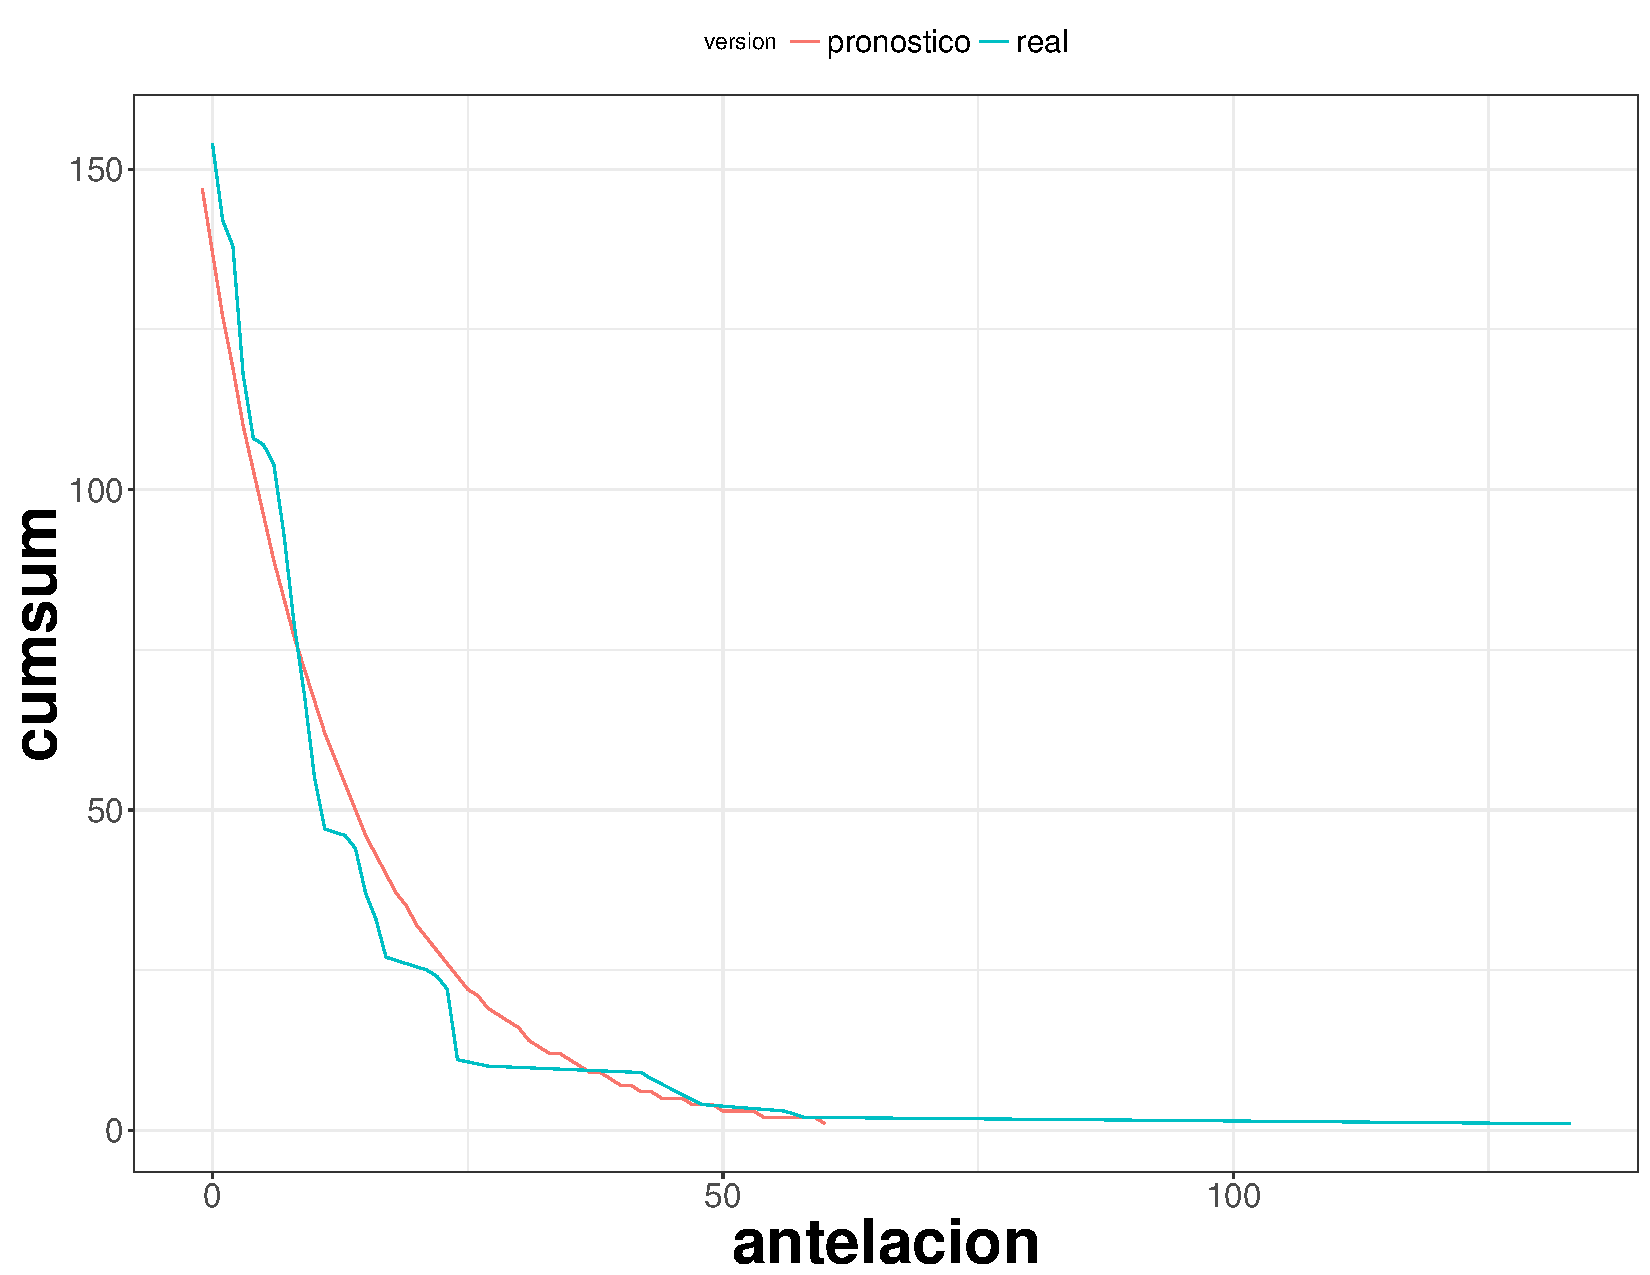
\includegraphics[width=\maxwidth,height=8cm]{figures/Resultados-2}  
  \caption{Curva de pickup real vs pronosticada (2)}
\end{figure}

\begin{figure}[H]
  \centering
      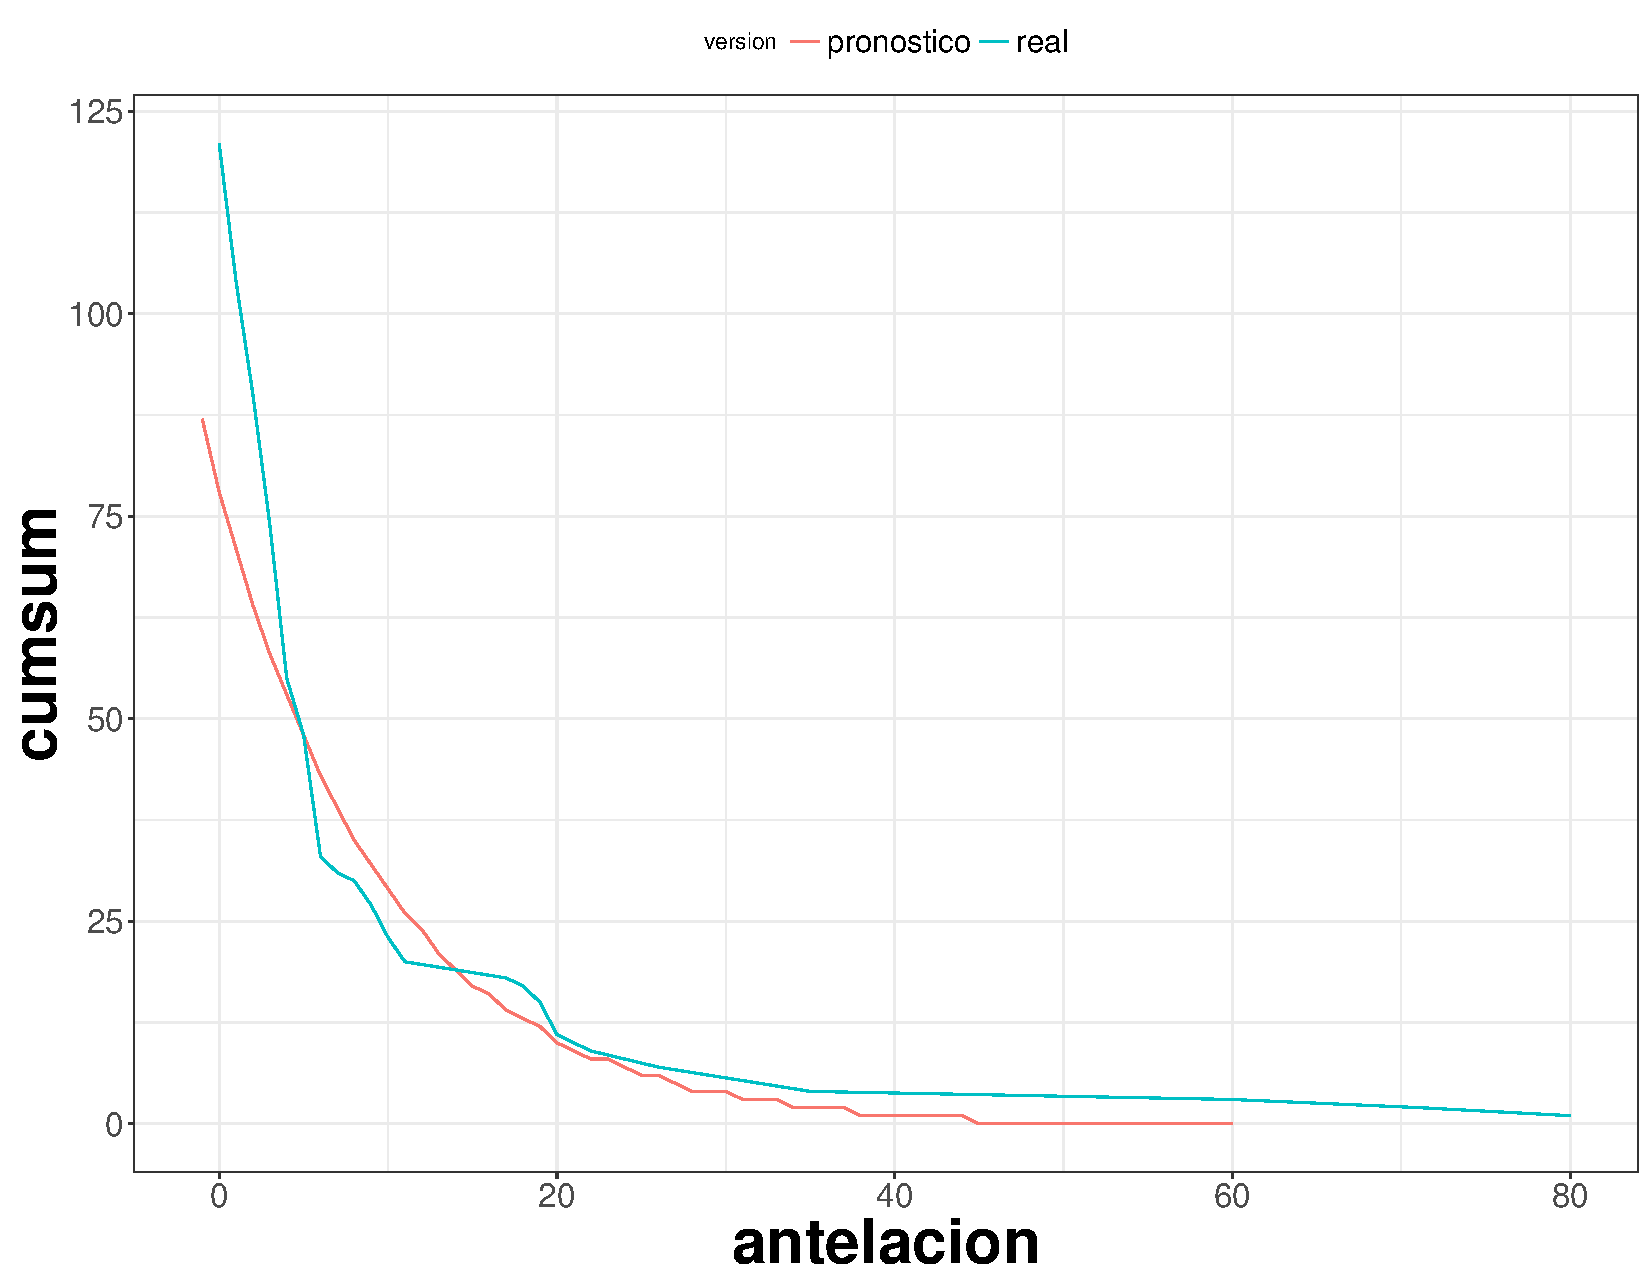
\includegraphics[width=\maxwidth,height=8cm]{figures/Resultados-3}  
  \caption{Curva de pickup real vs pronosticada (3)}
\end{figure}

\begin{figure}[H]
  \centering
      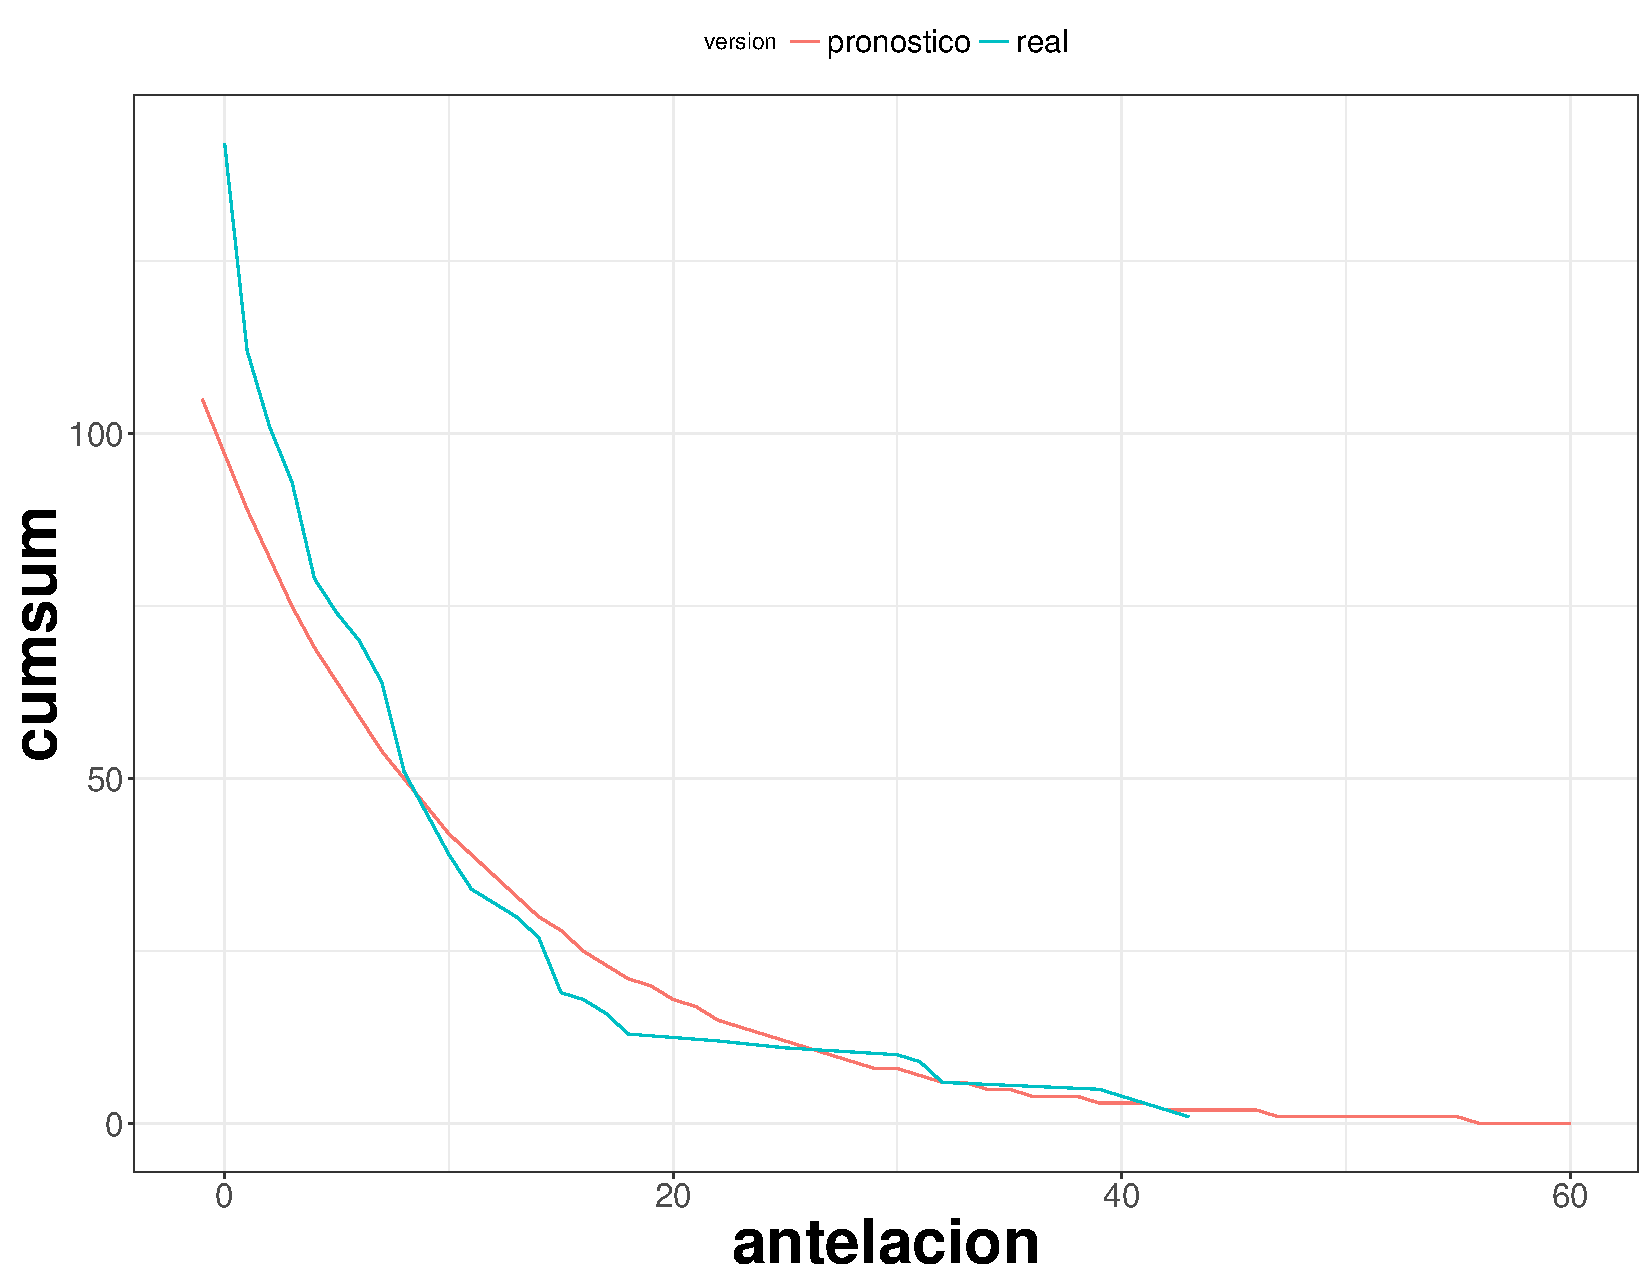
\includegraphics[width=\maxwidth,height=10cm]{figures/Resultados-4}  
  \caption{Curva de pickup real vs pronosticada (4)}
\end{figure}

Podemos observar que la curva pronosticada tiene un buen ajuste sobre la curva real en la mayoría de los casos.

Para realizar la validación del modelo se dividió el data set en dos partes, la primera parte se utilizó para el entrenamiento del modelo y la segunda parte para la validación del mismo, de esta forma se pudo comparar el pronóstico de demanda arrojado por el modelo contra la demanda real de la propiedad en 220 días para el año 2018.

Para evaluar el desempeño del modelo se utilizó la medida \emph{MAPE} definida como: $$MAPE=\frac{1}{n}\sum_{t=1}^{n}|\frac{y_t-h_t}{y_t}|$$

Dónde:
\begin{itemize}[noitemsep]
  \item n = Número de puntos ajustados
  \item $y_t$ = Cuartos noche vendidos en el tiempo $t$
  \item $h_t$ = Venta de cuartos noche pronósticada en el tiempo $t$
\end{itemize}


El \emph{MAPE} observado durante la validación del modelo fue de 17.67\% que de acuerdo con la investigación realizada en el capítulo dos está dentro de los parámetros aceptables.

\subsection*{Modelo de regresión de Ridge}

\subsection*{Modelo de análisis de series temporales ARIMA}

\subsection*{Modelo de maximización de ingresos}

El modelo de recomendaciones de precio toma como entrada la demanda pronósticada por el módelo de pronóstico de demanda. A partir de ahi, se define un problema de maximización sujeto a restricciones y se arroja una matriz que contiene los precios para un tipo de cuarto dependiendo del inventario disponible dentro de la propidad.

A continuación se muestra un extracto del resultado:

\begin{table}[H]
  \centering
  \csvautotabular{data/rates.csv}\par
  \caption{Matriz de asignacion de precio por inventario disponible}
\end{table}

La manera en la que se debe interpretar esta matriz es la siguiente: Para el día 7 de Julio de 2018, las habitaciones sencillas de este hotel deben de tener un precio de \$784.76 MXN si el inventario disponible esta entre 121 y 159 habitaciones disponibles. Si se tienen entre 81 y 120 habitaciones disponibles, el precio debe de ser de \$903.32 MXN y así sucesivamente. De esta manera podemos asignar un lote de habitaciones a diferentes rangos de precios siendo las últimas habitaciones disponibles las que tengan el precio más alto.


A continuación se presenta una gráfica con los resultados obtenidos por el modelo de maximización de ingresos:

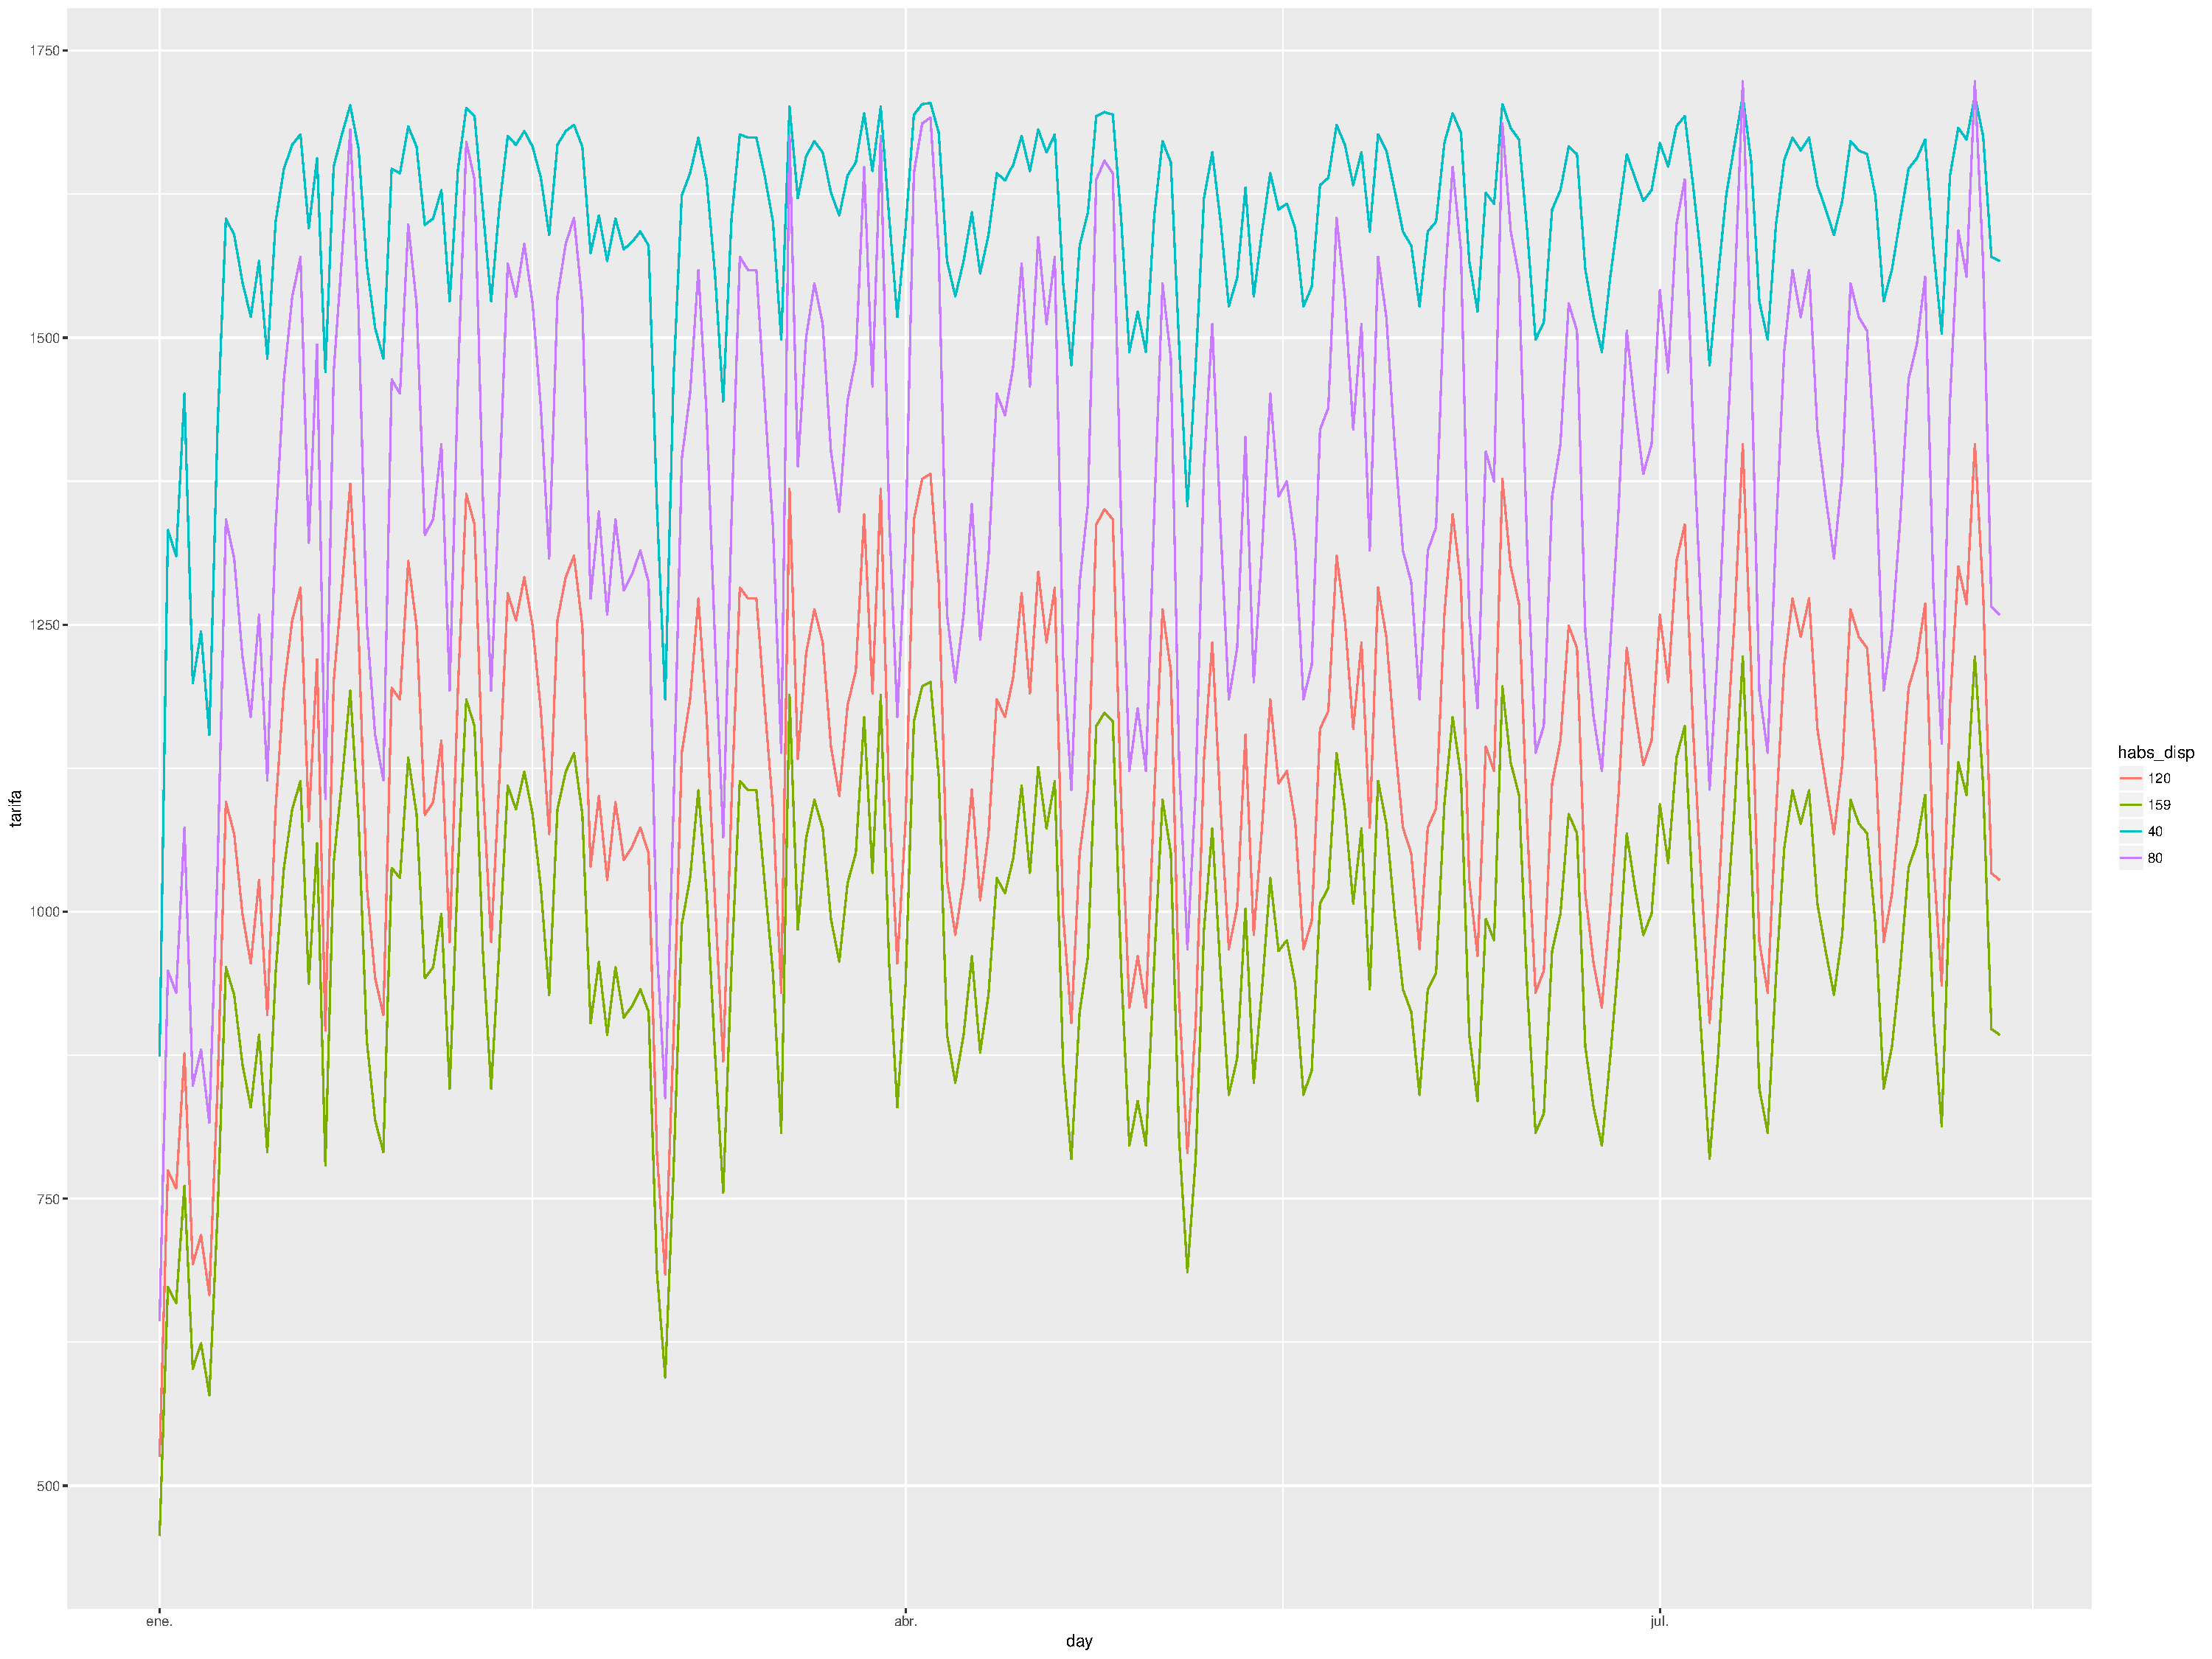
\includegraphics[width=\maxwidth]{figures/Pricing_graph-1} 

Para medir el desempeño del modelo de maximización de ingresos, se tomaron los resultados y se calcularon las tarifas promedio a partir de los datos obtenidos y se compararon contra las tarifas promedio reportadas por la propiedad para el año 2018.

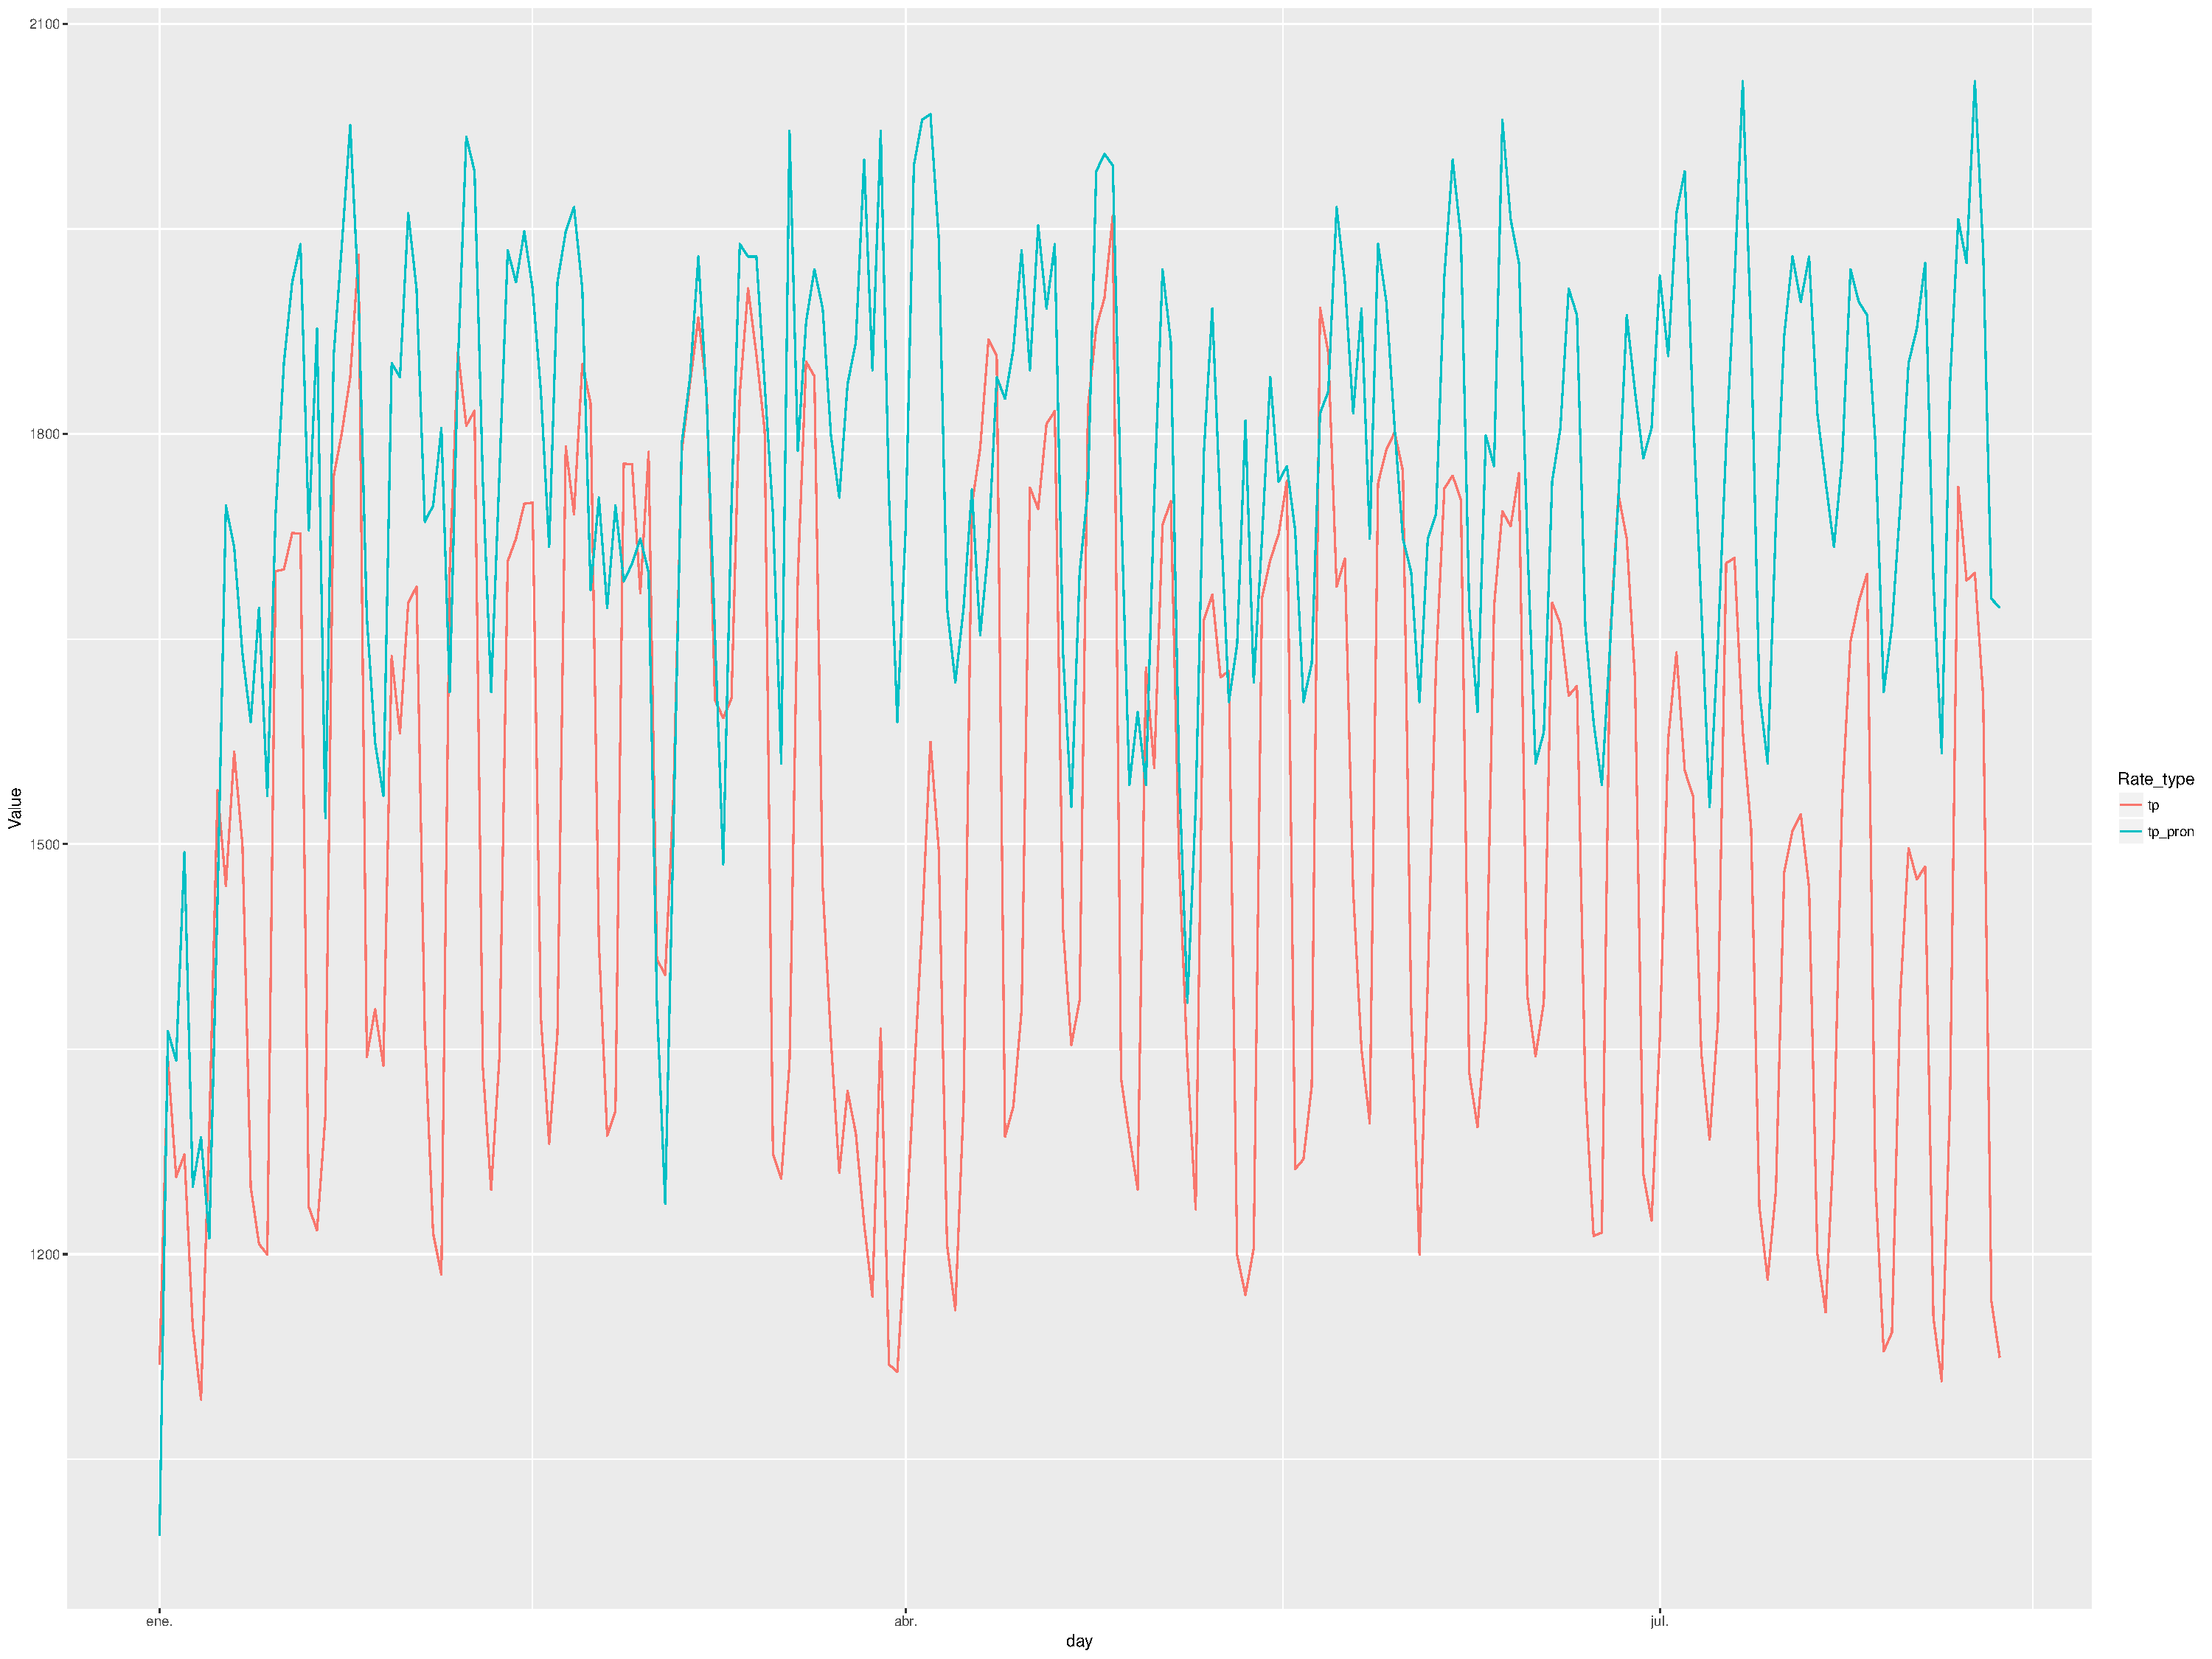
\includegraphics[width=\maxwidth]{figures/Pricing-1} 

Si obtenemos la diferencia de tarifas promedio, notamos que si se utilizara el resultado del modelo de optimización tendríamos un aumento en los ingresos de aproximadamente 57555.70 MXN. Sin embargo, para poder validar este resultado se propone implementar este modelo dentro de la propiedad y comprobar sus resultados en la operación.




